\documentclass{article}
\usepackage[T1]{fontenc}
\usepackage{lmodern}
\usepackage{graphicx}
\usepackage{amsmath,amssymb}
\usepackage[a4paper,margin=2cm]{geometry}
\usepackage[absolute,overlay]{textpos}
\setlength{\TPHorizModule}{1mm}
\setlength{\TPVertModule}{1mm}
\usepackage[indonesian]{babel}
\usepackage{hyperref}
\setlength{\emergencystretch}{2em}
% unit: Halaman 78

\begin{document}

% === Halaman 78 (llm) ===

\begin{verbatim}
def ProgramSteganografi():
    print("-- Steganografi pada Citra Digital --")
    print("1: Penyisipan pesan")
    print("2: Ekstraksi pesan")

\vspace{136.62mm}

    pilih = input()
    if pilih == '1':
        print("Masukkan nama citra cover (beserta path-nya")
        cover = input()
        print("Ketikkan pesan yang akan disisipkan ke dalam citra")
        pesan = input()
        print("Masukkan nama citra output (stego image) beserta path-nya")
        stego = input()
        print("Penyisipan pesan...")
        EmbeddingPesan(cover, pesan, stego)
    elif pilih == '2':
        print("Masukkan nama citra stego beserta path-nya")
        stego = input()
        print("Ekstraksi pesan...")
        EkstraksiPesan(stego)
    else:
        print("Pilihan salah")
\end{verbatim}

% deskripsi: Screenshot blok kode Python untuk program steganografi citra digital
% bbox normalisasi: [0.0400, 0.4100, 0.9400, 0.8700]
\begin{textblock*}{189.00mm}(8.40mm,121.77mm)
\noindent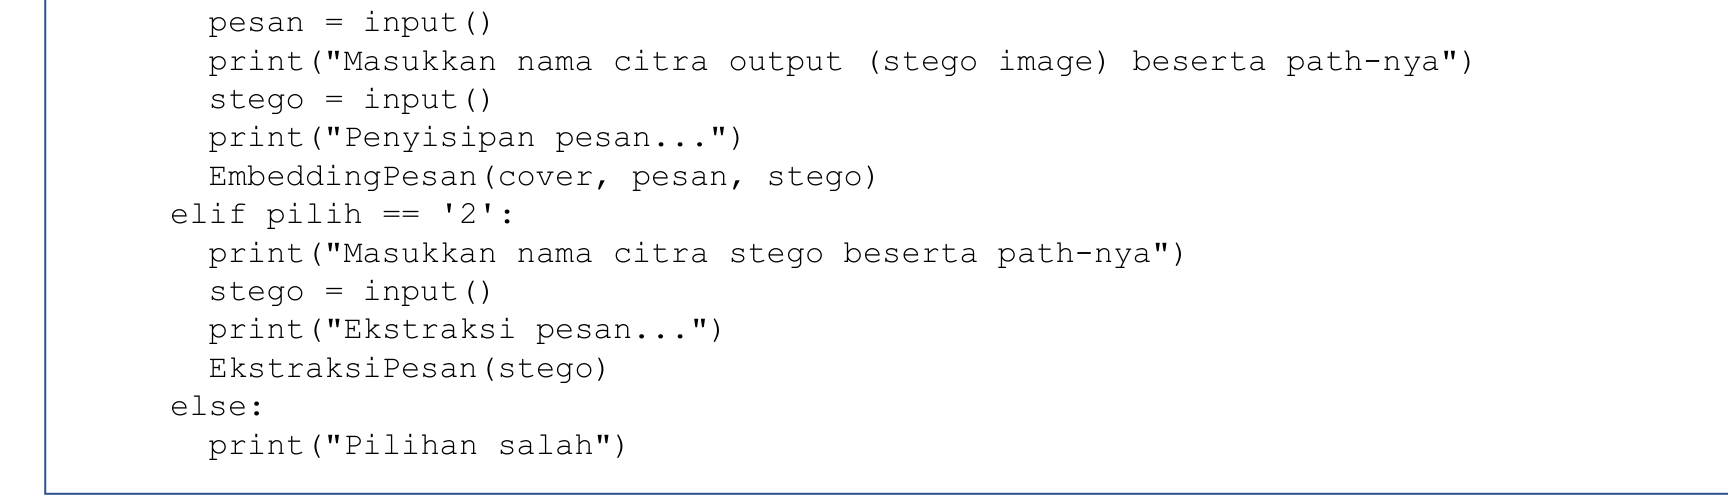
\includegraphics[width=189.00mm,height=136.62mm]{../../images/llm/page_078_img_01.png}%
\end{textblock*}

\end{document}
